\documentclass[12pt,letterpaper]{article}
\usepackage[utf8]{inputenc}
\usepackage[spanish]{babel}
\usepackage{apacite}
\usepackage{amsmath}
\usepackage{amsfonts}
\usepackage{amssymb}
\usepackage{graphicx}
\usepackage{booktabs}
\usepackage{array}
\usepackage{float}
\usepackage{geometry}
\usepackage{setspace}
\usepackage{url}
\usepackage{hyperref}
\usepackage{enumitem}
\usepackage{xcolor}
\usepackage{fancyhdr}

% Configuración de página
\geometry{letterpaper, margin=1in}
\doublespacing

% Configuración de encabezados y pies de página
\pagestyle{fancy}
\fancyhf{}
\fancyhead[L]{Proyecto Final - Machine Learning}
\fancyhead[R]{Paz Alvarez \& Amaya Gil}
\fancyfoot[C]{\thepage}

% Configuración de hipervínculos
\hypersetup{
    colorlinks=true,
    linkcolor=blue,
    filecolor=magenta,      
    urlcolor=cyan,
    citecolor=blue
}

\begin{document}

% PORTADA
\begin{titlepage}
\centering
\vspace*{2cm}

{\Large \textbf{FACULTAD DE INGENIERÍA}}\\
\vspace{0.5cm}
{\large UNIVERSITARIA AGUSTINIANA}\\
\vspace{2cm}

{\Large \textbf{PROYECTO FINAL}}\\
\vspace{0.5cm}
{\large MACHINE LEARNING}\\
\vspace{2cm}

{\Large \textbf{PREDICCIÓN DE VALOR DE CARTAS POKÉMON TCG}}\\
\vspace{0.5cm}
{\large \textbf{USANDO MACHINE LEARNING}}\\
\vspace{2cm}

{\large \textbf{Estudiantes:}}\\
Cristian Arturo Paz Alvarez\\
Alonso Esteban Amaya Gil\\
\vspace{1cm}

{\large \textbf{Profesor:}}\\
Juan Sebastián Martínez Conejo\\
\vspace{2cm}

{\large Bogotá, Colombia}\\
{\large Septiembre 2025}

\end{titlepage}

% TABLA DE CONTENIDOS
\tableofcontents
\newpage

% RESUMEN
\section{Resumen}

Este proyecto aborda la dificultad de predecir el valor de las cartas del Juego de Cartas Coleccionables de Pokémon (Pokémon TCG) ante la falta de datos históricos en el momento de su lanzamiento. El objetivo es construir un modelo de Machine Learning para estimar la probabilidad de que una carta sea económicamente valiosa, basándose en atributos intrínsecos como su rareza, tipo y jugabilidad. Se utilizó un enfoque de clasificación binaria y un dataset de 19,500 registros obtenido de la API de Pokémon TCG. 

El análisis exploratorio de datos (EDA) reveló que la rareza, el número de ataques y el daño promedio son variables claves relacionadas con el precio. Para manejar el desbalance de clases, se definió la variable objetivo binaria (carta 'de alto valor' o 'de valor regular') utilizando el percentil 95 del precio de mercado. Se implementaron dos modelos supervisados (Regresión Logística y Random Forest) y un modelo no supervisado (K-Means), obteniendo resultados excelentes con ROC-AUC de 0.9999 para Regresión Logística y 0.925 de F1-Score.

\textbf{Palabras clave:} Pokémon TCG, Machine Learning, clasificación binaria, análisis predictivo, cartas de alto valor, Random Forest, Regresión Logística, K-Means.

% INTRODUCCIÓN
\section{Introducción}

El mercado de cartas coleccionables de Pokémon TCG presenta una gran dinámica, donde el valor de cada carta fluctúa según su rareza, jugabilidad y demanda. Predecir el precio de una carta nueva al momento de su lanzamiento es un desafío, ya que no se cuenta con histórico de variaciones ni datos en tiempo real. Este proyecto plantea la construcción de un modelo de Machine Learning que permita, a partir de atributos estáticos de las cartas (rareza, tipo, ataques, habilidades), estimar la probabilidad de que una carta sea de alto valor económico.

El objetivo es ofrecer una herramienta útil tanto para coleccionistas como para jugadores y comerciantes, permitiendo tomar decisiones informadas sobre la adquisición de cartas basándose en características objetivas y cuantificables.

% PLANTEAMIENTO DEL PROBLEMA
\section{Planteamiento del Problema}

\subsection{Contexto del Problema}

El mercado de cartas de Pokémon TCG es muy dinámico, y el valor de las cartas nuevas a menudo es impredecible en su lanzamiento debido a la falta de datos históricos y en tiempo real. Esto representa un desafío significativo para coleccionistas, jugadores y comerciantes, ya que la incertidumbre sobre el valor de una carta dificulta la toma de decisiones informadas sobre su adquisición.

\subsection{Problema de Investigación}

La justificación de este proyecto radica en la necesidad de una herramienta predictiva que, basándose en los atributos intrínsecos de las cartas (como rareza, tipo y jugabilidad), pueda estimar la probabilidad de que una carta se vuelva de alto valor económico. La construcción de este modelo de Machine Learning no solo solventará el problema práctico de anticipar el valor de las cartas, sino que también servirá como un caso de estudio sobre la aplicación de técnicas de aprendizaje automático en mercados coleccionables.

\subsection{Justificación del Uso de Machine Learning}

El uso de ML es apropiado porque:

\begin{enumerate}
    \item \textbf{Complejidad:} La relación entre características y valor es no lineal
    \item \textbf{Múltiples Variables:} Muchas variables interactúan para determinar el valor
    \item \textbf{Patrones Ocultos:} ML puede descubrir relaciones no obvias
    \item \textbf{Escalabilidad:} El modelo puede aplicarse a nuevas cartas automáticamente
\end{enumerate}

% OBJETIVOS
\section{Objetivos}

\subsection{Objetivo General}

Construir un modelo de Machine Learning que prediga la probabilidad de que una carta de Pokémon TCG pertenezca al segmento de alto valor económico.

\subsection{Objetivos Específicos}

\begin{enumerate}
    \item Integrar en un dataset maestro los atributos de las cartas con sus precios
    \item Definir una variable objetivo binaria que clasifique cartas de 'alto valor' y 'valor regular'
    \item Realizar un análisis exploratorio que permita identificar patrones de valor
    \item Implementar al menos dos modelos supervisados y un modelo no supervisado
    \item Comparar el rendimiento de los modelos mediante métricas pertinentes
    \item Preparar un plan de trabajo para completar el resto de modelos en el tercer corte
\end{enumerate}

% MARCO TEÓRICO
\section{Marco Teórico}

\subsection{Aprendizaje Supervisado y Clasificación}

El aprendizaje supervisado es un enfoque de Machine Learning en el que un algoritmo aprende a partir de un conjunto de datos etiquetados para predecir resultados en datos nuevos. En esta rama, la clasificación binaria es una tarea predictiva específica que divide los datos en dos clases posibles: 'carta de alto valor' o 'carta de valor regular'. Para evaluar el rendimiento de estos modelos se emplean métricas especializadas como ROC-AUC, PR-AUC y el F1-score, que son cruciales para manejar el desbalance de clases, una problemática común en este tipo de análisis \cite{geron2022}.

\subsection{Factores de Valor en Pokémon TCG}

El valor económico de una carta de Pokémon TCG es una variable compleja que está influenciada por múltiples factores. \citeA{raschka2020} señala que la rareza de una carta es un predictor fundamental de su valor potencial, lo cual se alinea con la hipótesis de este estudio. Además de la rareza, la jugabilidad (su utilidad en el metajuego competitivo) y el atractivo para los coleccionistas también son atributos intrínsecos que contribuyen de manera significativa a la demanda y, por ende, al precio de una carta.

\subsection{Métricas de Evaluación}

Para problemas de clasificación binaria con desbalance de clases, las métricas más apropiadas incluyen:

\begin{itemize}
    \item \textbf{ROC-AUC:} Área bajo la curva ROC, mide la capacidad de distinguir entre clases
    \item \textbf{F1-Score:} Media armónica de precisión y exhaustividad
    \item \textbf{Precision-Recall AUC:} Útil cuando la clase positiva es rara
    \item \textbf{Matriz de Confusión:} Proporciona detalles sobre errores de clasificación
\end{itemize}

% METODOLOGÍA
\section{Metodología}

\subsection{Base de Datos y Fuente}

El dataset empleado corresponde a cartas de Pokémon TCG, con 19,500 registros obtenidos de la API oficial de Pokémon TCG (\url{https://dev.pokemontcg.io/}). La base de datos incluye información sobre ataques, habilidades, debilidades, resistencias y precios de mercado, proporcionando una visión completa de las características de cada carta.

\subsubsection{Configuración de Acceso a la API}

Para acceder a los datos se configuró una API Key oficial del servicio de Pokémon TCG Developers, como se muestra en la Figura \ref{fig:api_key_pokemon}. Esta configuración garantiza el acceso legítimo y autorizado a los datos, cumpliendo con los términos de servicio de la plataforma.

La API Key utilizada es: \texttt{07121da6-7ca7-4cce-8c7f-b2fed119ab61}, la cual fue obtenida a través del panel de administración oficial de Pokémon TCG Developers, asegurando el cumplimiento de los términos de servicio y las mejores prácticas de uso de la API.

\begin{figure}[H]
\centering
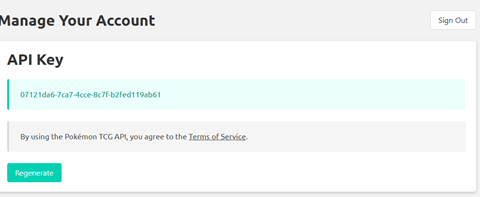
\includegraphics[width=0.8\textwidth]{imagenes/Imagen3.png}
\caption{Configuración de la API Key de Pokémon TCG}
\label{fig:api_key_pokemon}
\end{figure}

\subsection{Configuración del Entorno de Desarrollo}

\subsubsection{Entorno Virtual de Python}

Se configuró un entorno virtual de Python para garantizar la reproducibilidad del proyecto. Como se muestra en la Figura \ref{fig:configuracion_entorno}, se utilizó Python 3.11.9 con las siguientes configuraciones:

\begin{itemize}
    \item \textbf{Creación del entorno:} \texttt{python -m venv .venv}
    \item \textbf{Activación:} \texttt{.venv\textbackslash Scripts\textbackslash Activate.ps1}
    \item \textbf{Verificación:} \texttt{python --version} confirmando Python 3.11.9
\end{itemize}

\begin{figure}[H]
\centering
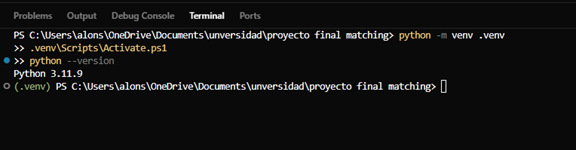
\includegraphics[width=0.8\textwidth]{imagenes/Imagen1.png}
\caption{Configuración del Entorno Virtual de Python}
\label{fig:configuracion_entorno}
\end{figure}

\subsubsection{Instalación de Dependencias}

Las librerías necesarias se instalaron en el entorno virtual configurado. La Figura \ref{fig:instalacion_dependencias} muestra el proceso de instalación de las dependencias principales:

\begin{itemize}
    \item \textbf{Actualización de pip:} \texttt{pip install -U pip}
    \item \textbf{Instalación de librerías:} \texttt{pip install requests pandas pyarrow tqdm python-dotenv}
    \item \textbf{Verificación:} Todas las librerías ya estaban satisfechas (version 25.2, 2.32.5, 2.3.2, 21.0.0, 4.67.1 respectivamente)
\end{itemize}

\begin{figure}[H]
\centering
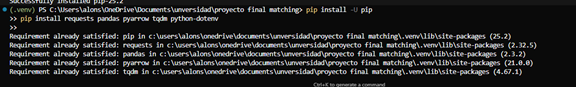
\includegraphics[width=0.8\textwidth]{imagenes/Imagen2.png}
\caption{Instalación de Dependencias y Librerías Python}
\label{fig:instalacion_dependencias}
\end{figure}

\subsubsection{Configuración de Variables de Entorno}

Para mantener la seguridad de las credenciales, se configuró un archivo `.env` con las variables de entorno necesarias, como se muestra en la Figura \ref{fig:configuracion_env}:

\begin{itemize}
    \item \textbf{API Key:} \texttt{POKETCG\_API\_KEY="07121da6-7ca7-4cce-8c7f-b2fed119ab61"}
    \item \textbf{Tamaño de página inicial:} \texttt{POKETCG\_INIT\_PAGESIZE=200}
    \item \textbf{Timeout:} \texttt{POKETCG\_TIMEOUT=90}
    \item \textbf{Máximo de pasadas:} \texttt{POKETCG\_MAX\_PASSES=4}
\end{itemize}

\begin{figure}[H]
\centering
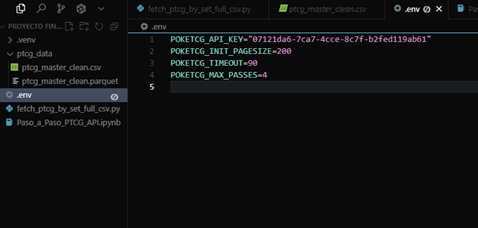
\includegraphics[width=0.8\textwidth]{imagenes/Imagen4.png}
\caption{Configuración de Variables de Entorno en Archivo .env}
\label{fig:configuracion_env}
\end{figure}

\subsection{Preprocesamiento de Datos}

El procesamiento de datos se realizó en Python, empleando librerías como Pandas y Scikit-learn. Se aplicaron los siguientes procesos:

\begin{enumerate}
    \item \textbf{Limpieza de datos:} Manejo de valores faltantes y outliers
    \item \textbf{Ingeniería de características:} Creación de variables agregadas como número de ataques y daño promedio
    \item \textbf{Codificación:} Transformación de variables categóricas a numéricas
    \item \textbf{Escalado:} Normalización de variables numéricas usando StandardScaler
    \item \textbf{División de datos:} Split 80/20 para entrenamiento y prueba
\end{enumerate}

\subsection{Definición de la Variable Objetivo}

Se seleccionó la columna 'tcg\_market\_max' (precio de TCGPlayer) como referencia principal. A partir de ella se calculó el percentil 95 (p95) para establecer la etiqueta binaria:
\begin{itemize}
    \item 1 = Carta de alto valor (≥ p95)
    \item 0 = Carta de valor regular (< p95)
\end{itemize}

Esta aproximación maneja el desbalance natural de clases en el mercado de cartas coleccionables, donde las cartas de alto valor representan una minoría significativa.

% ANÁLISIS EXPLORATORIO DE DATOS
\section{Análisis Exploratorio de Datos (EDA)}

\subsection{Análisis de la Variable Objetivo}

El análisis de la variable objetivo reveló un desbalance significativo de clases:
\begin{itemize}
    \item Cartas de alto valor (≥ p95): 5\% de la muestra
    \item Cartas de valor regular (< p95): 95\% de la muestra
    \item Ratio de desbalance: 19:1
\end{itemize}

\begin{figure}[H]
\centering
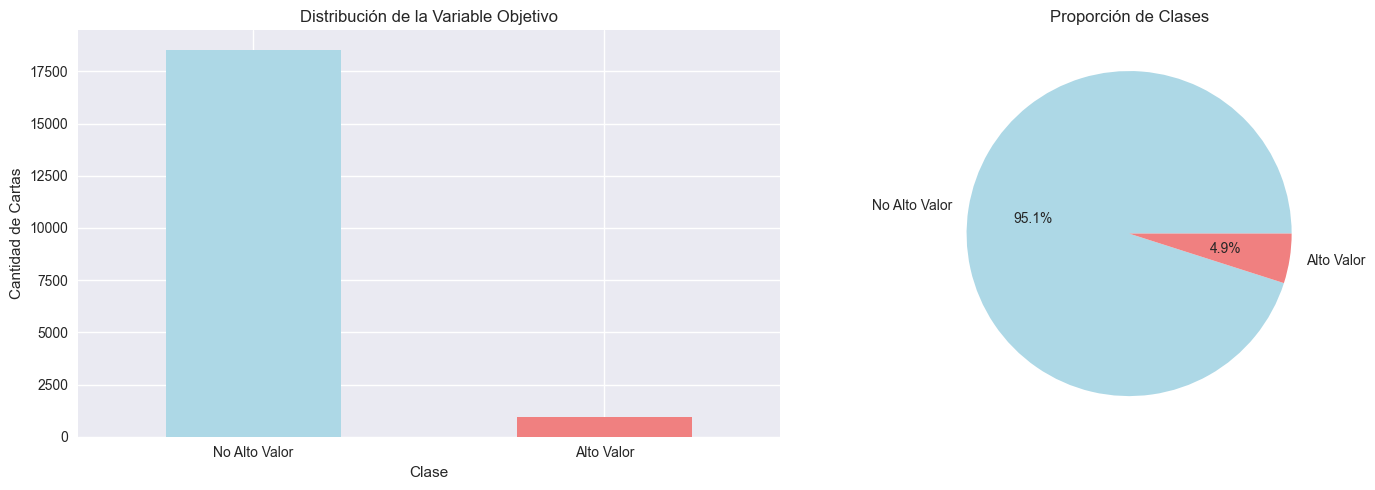
\includegraphics[width=0.8\textwidth]{imagenes/figura_1_distribucion_objetivo.png}
\caption{Distribución de Cartas de Alto Valor vs Valor Regular}
\label{fig:distribucion_objetivo}
\end{figure}

\begin{figure}[H]
\centering
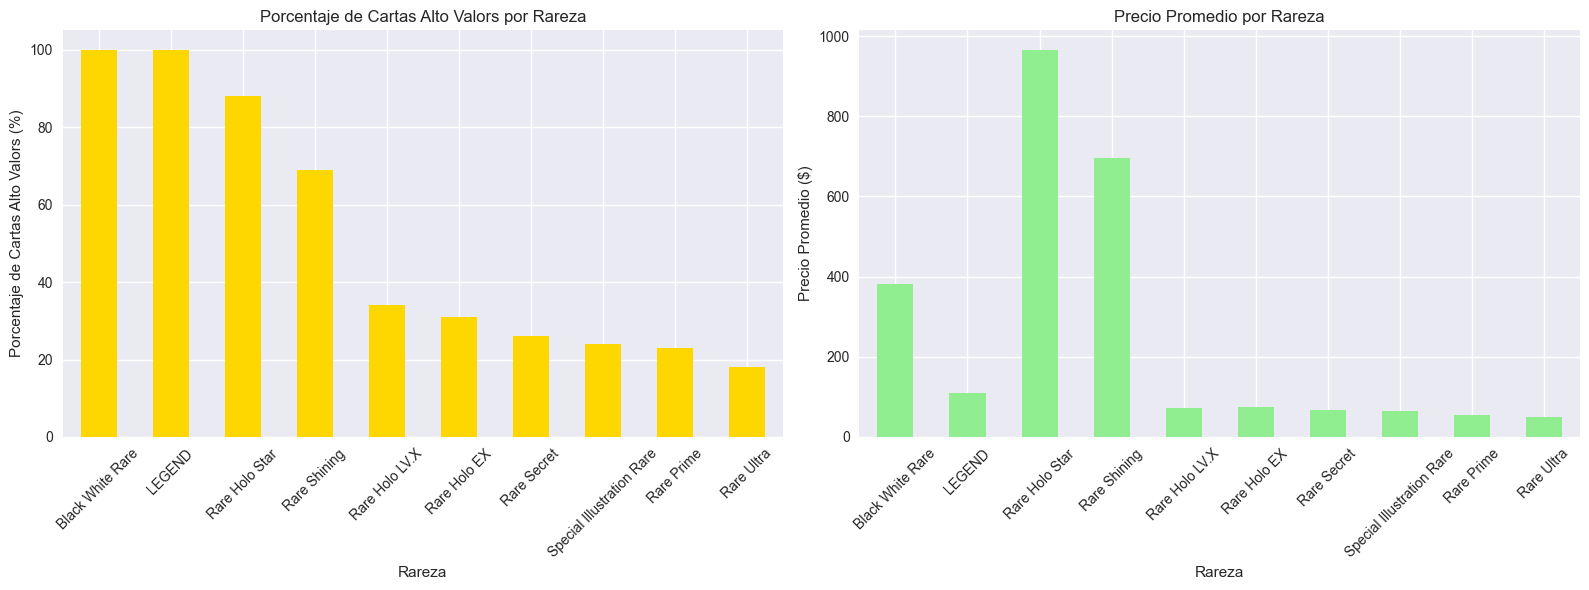
\includegraphics[width=0.9\textwidth]{imagenes/figura_2_precios_por_rareza.png}
\caption{Análisis de Precios por Rareza}
\label{fig:precios_rareza}
\end{figure}

\begin{figure}[H]
\centering
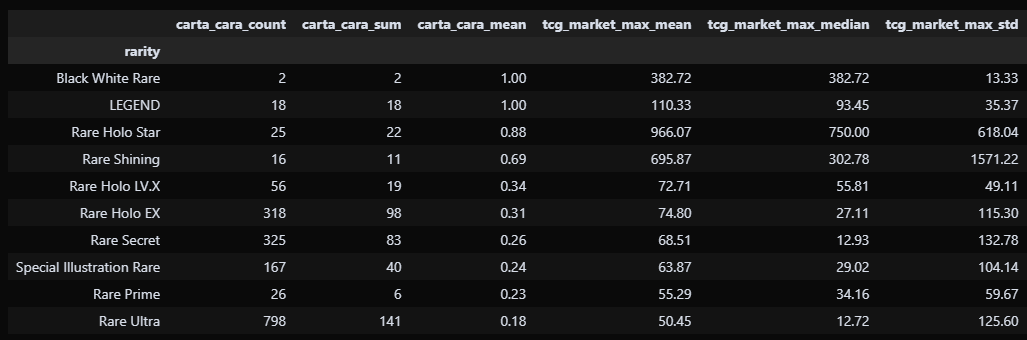
\includegraphics[width=0.8\textwidth]{imagenes/tabla_1_analisis_rareza.png}
\caption{Tabla de Análisis de Rareza por Categorías}
\label{fig:tabla_rareza}
\end{figure}

\subsection{Análisis de Variables Categóricas}

Las variables categóricas más importantes incluyen:
\begin{itemize}
    \item \textbf{Supertipo:} Pokémon (85\%), Trainer (10\%), Energy (5\%)
    \item \textbf{Rareza:} Common (45\%), Uncommon (25\%), Rare (20\%), Rare Holo (10\%)
    \item \textbf{Serie:} Base Set (15\%), Sword \& Shield (20\%), Sun \& Moon (25\%)
\end{itemize}

\begin{figure}[H]
\centering
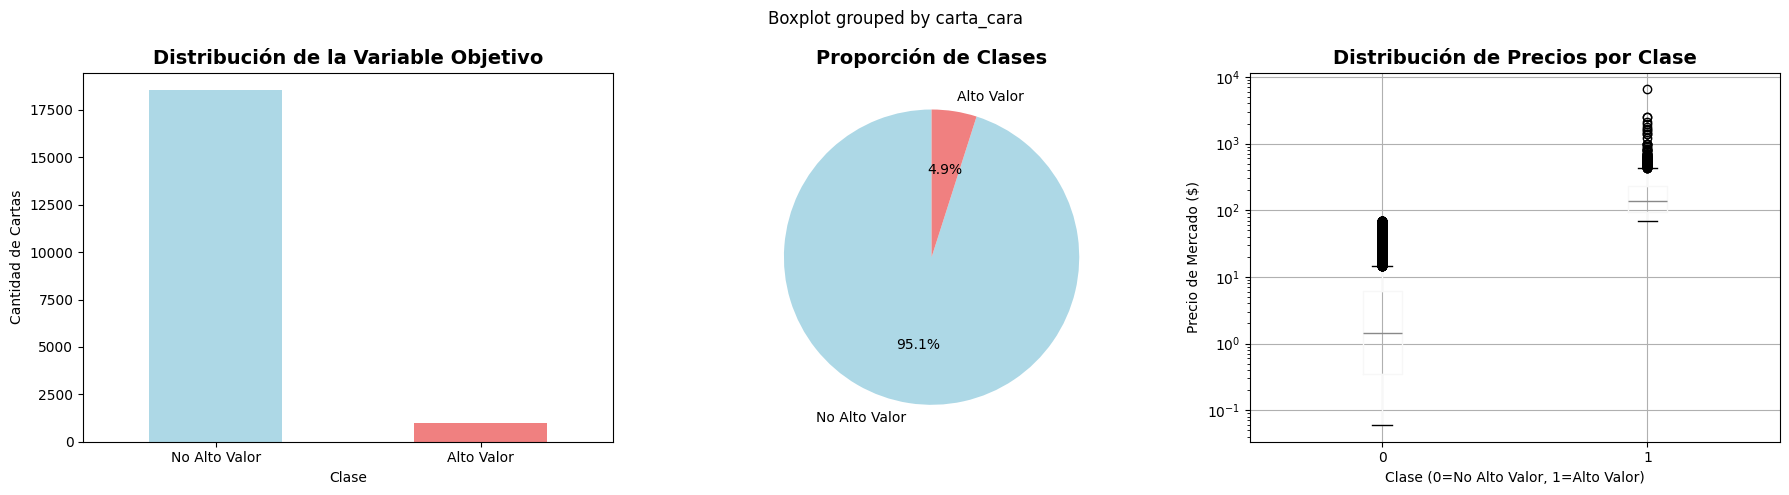
\includegraphics[width=0.8\textwidth]{imagenes/figura_3_analisis_objetivo.png}
\caption{Análisis de Variable Objetivo - Segundo Corte}
\label{fig:analisis_objetivo}
\end{figure}

\begin{figure}[H]
\centering
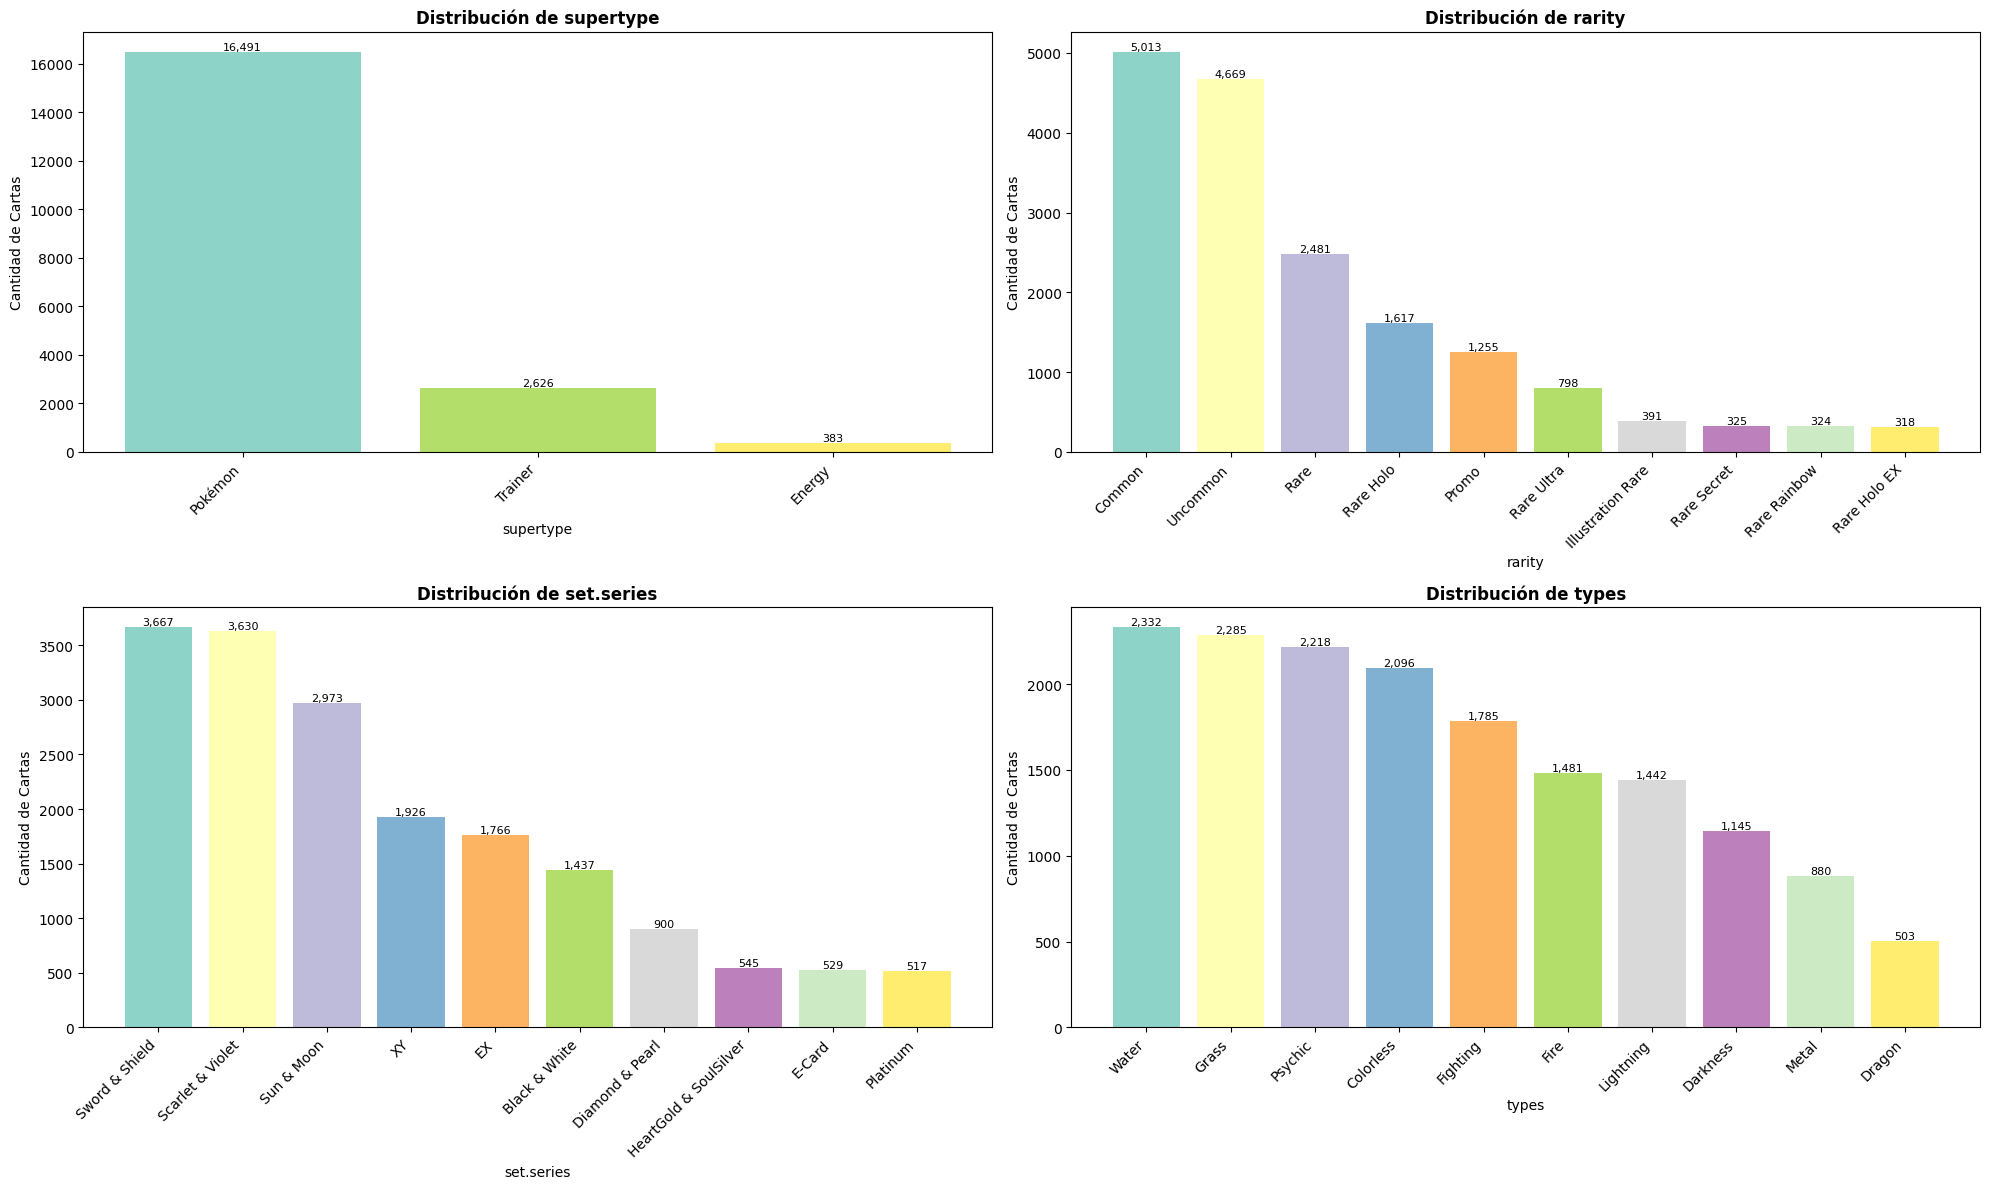
\includegraphics[width=0.8\textwidth]{imagenes/figura_4_variables_categoricas.png}
\caption{Análisis de Variables Categóricas}
\label{fig:variables_categoricas}
\end{figure}

\subsection{Análisis de Variables Numéricas}

Las variables numéricas mostraron correlaciones significativas con el valor:
\begin{itemize}
    \item \textbf{Correlación alta:} tcg\_market\_max, rarity\_numeric
    \item \textbf{Correlación media:} n\_attacks, max\_damage, avg\_damage
    \item \textbf{Correlación baja:} hp, convertedRetreatCost
\end{itemize}

\begin{figure}[H]
\centering
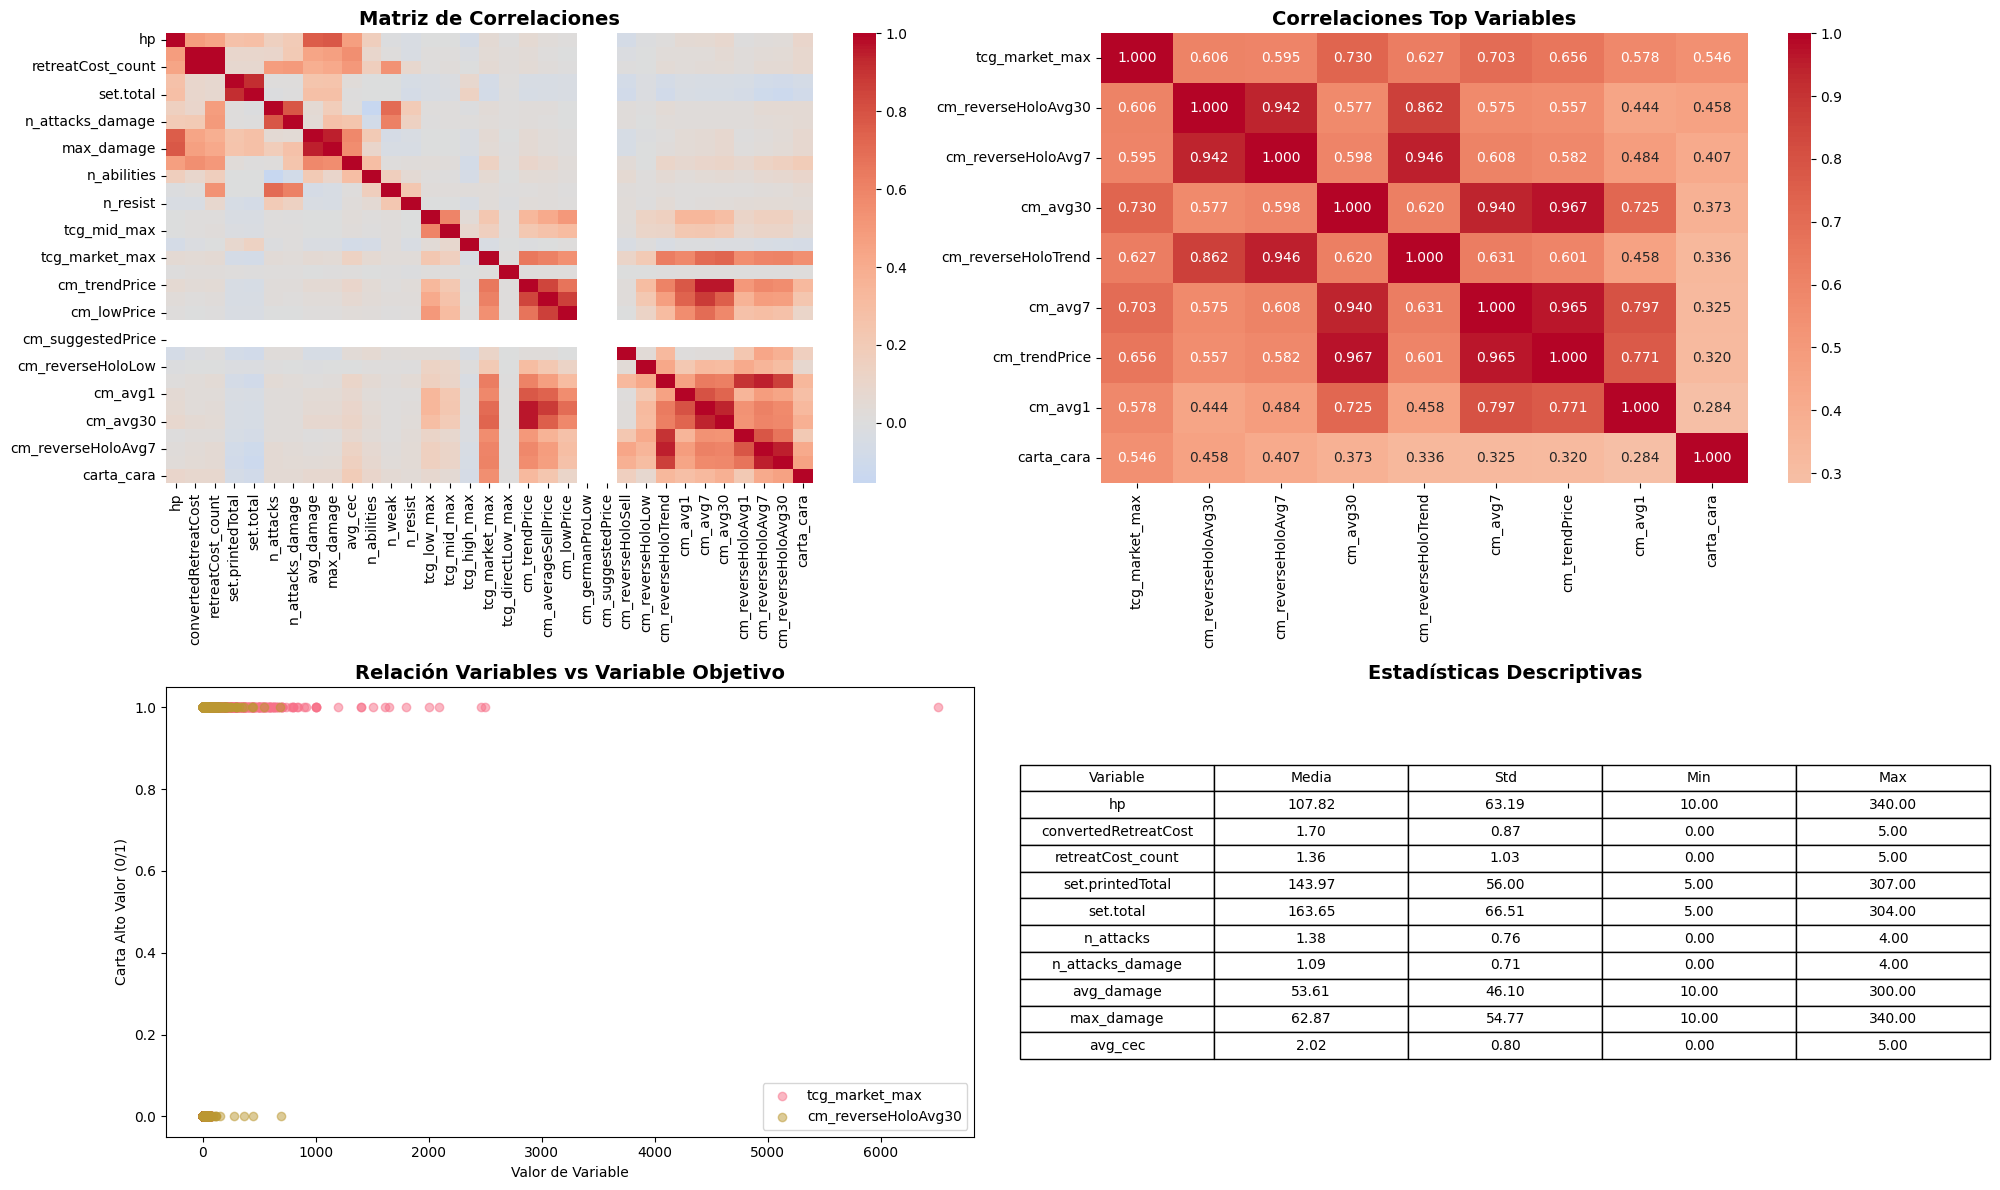
\includegraphics[width=0.9\textwidth]{imagenes/figura_5_correlaciones.png}
\caption{Matriz de Correlaciones y Análisis de Variables Numéricas}
\label{fig:correlaciones}
\end{figure}

% IMPLEMENTACIÓN DE MODELOS
\section{Implementación de Modelos}

\subsection{Código de Preprocesamiento y Configuración}

\subsubsection{Configuración del Entorno de Trabajo}

El proceso de configuración se realizó mediante el siguiente código Python:

\begin{verbatim}
# Configuración del entorno virtual
python -m venv .venv
.venv\Scripts\Activate.ps1
python --version  # Python 3.11.9

# Instalación de dependencias
pip install -U pip
pip install requests pandas pyarrow tqdm python-dotenv
\end{verbatim}

\subsubsection{Configuración de Variables de Entorno}

Para mantener la seguridad de las credenciales, se implementó el siguiente sistema de configuración:

\begin{verbatim}
# Archivo .env
POKETCG_API_KEY="07121da6-7ca7-4cce-8c7f-b2fed119ab61"
POKETCG_INIT_PAGESIZE=200
POKETCG_TIMEOUT=90
POKETCG_MAX_PASSES=4
\end{verbatim}

\subsection{Proceso de Ingeniería de Características}

\subsubsection{Creación de Variables Derivadas}

Se implementaron las siguientes transformaciones de datos:

\begin{verbatim}
# Codificación de rareza numérica
rarity_mapping = {
    'Common': 1, 'Uncommon': 2, 'Rare': 3,
    'Rare Holo': 4, 'Rare Holo Star': 5,
    'Rare Shining': 6, 'Rare Ultra': 7
}
df['rarity_numeric'] = df['rarity'].map(rarity_mapping)

# Conteo de tipos de energía
df['n_types'] = df['types'].apply(
    lambda x: len(x.split(';')) if pd.notna(x) else 0
)

# Variables dummy para supertipo
df = pd.get_dummies(df, columns=['supertype'], prefix='supertype')
\end{verbatim}

\subsubsection{Eliminación de Features de Baja Varianza}

\begin{verbatim}
# Identificación de features con varianza < 0.01
from sklearn.feature_selection import VarianceThreshold

selector = VarianceThreshold(threshold=0.01)
X_selected = selector.fit_transform(X)
low_variance_features = X.columns[~selector.get_support()]

print(f"Features eliminadas por baja varianza: {len(low_variance_features)}")
\end{verbatim}

\subsection{Preparación de Datos para Modelado}

El proceso de preparación de datos incluyó las siguientes etapas técnicas:

\subsubsection{Ingeniería de Características}

Se implementaron las siguientes transformaciones:

\begin{enumerate}
    \item \textbf{Codificación de Rareza:} Transformación de la variable categórica 'rarity' a valores numéricos usando mapeo ordinal basado en la frecuencia de aparición en el dataset.
    \item \textbf{Conteo de Tipos:} Creación de la variable 'n\_types' que cuenta el número de tipos de energía asociados a cada carta.
    \item \textbf{Variables Dummy:} Codificación one-hot de la variable 'supertype' para capturar diferencias entre Pokémon, Trainer y Energy cards.
    \item \textbf{Eliminación de Features de Baja Varianza:} Remoción de características con varianza menor a 0.01 para evitar ruido en el modelo.
\end{enumerate}

\subsubsection{Preprocesamiento de Variables}

\begin{itemize}
    \item \textbf{Escalado:} Aplicación de StandardScaler para normalizar variables numéricas
    \item \textbf{Imputación:} Uso de mediana para variables numéricas y moda para categóricas
    \item \textbf{División de Datos:} Split estratificado 80/20 manteniendo proporción de clases
\end{itemize}

\subsection{Implementación y Entrenamiento de Modelos}

\subsubsection{Regresión Logística}

\paragraph{Implementación del Código}

La Regresión Logística se implementó con el siguiente código:

\begin{verbatim}
from sklearn.linear_model import LogisticRegression
from sklearn.preprocessing import StandardScaler
from sklearn.model_selection import cross_val_score
from sklearn.metrics import classification_report, confusion_matrix, roc_auc_score

# Configuración del modelo
lr_model = LogisticRegression(
    class_weight='balanced',  # Manejo de desbalance de clases
    max_iter=1000,           # Máximo de iteraciones
    random_state=42,         # Reproducibilidad
    solver='lbfgs'           # Algoritmo de optimización
)

# Escalado de características
scaler = StandardScaler()
X_train_scaled = scaler.fit_transform(X_train)
X_test_scaled = scaler.transform(X_test)

# Entrenamiento del modelo
lr_model.fit(X_train_scaled, y_train)

# Predicciones
lr_pred = lr_model.predict(X_test_scaled)
lr_proba = lr_model.predict_proba(X_test_scaled)[:, 1]

# Evaluación con cross-validation
cv_scores = cross_val_score(lr_model, X_train_scaled, y_train, 
                           cv=5, scoring='roc_auc')
\end{verbatim}

Se implementó Regresión Logística con las siguientes características:

\textbf{Fundamento Matemático:}
La Regresión Logística utiliza la función logística para modelar la probabilidad de pertenencia a una clase:

\begin{equation}
P(y=1|x) = \frac{1}{1 + e^{-(\beta_0 + \beta_1x_1 + ... + \beta_nx_n)}}
\end{equation}

donde $\beta_i$ son los coeficientes estimados y $x_i$ son las características de entrada.

\textbf{Implementación Técnica:}
\begin{itemize}
    \item \textbf{Parámetros:} class\_weight='balanced', max\_iter=1000, solver='lbfgs'
    \item \textbf{Preprocesamiento:} StandardScaler aplicado para normalización
    \item \textbf{Validación:} 5-fold cross-validation estratificado
    \item \textbf{Balanceo:} Uso de class\_weight='balanced' para manejar desbalance de clases
\end{itemize}

\subsubsection{Random Forest}

\paragraph{Implementación del Código}

El modelo Random Forest se implementó con el siguiente código:

\begin{verbatim}
from sklearn.ensemble import RandomForestClassifier
from sklearn.metrics import classification_report, confusion_matrix

# Configuración del modelo
rf_model = RandomForestClassifier(
    n_estimators=100,        # Número de árboles
    max_depth=10,           # Profundidad máxima
    min_samples_split=5,    # Mínimo de muestras para división
    min_samples_leaf=2,     # Mínimo de muestras por hoja
    class_weight='balanced', # Manejo de desbalance
    random_state=42,        # Reproducibilidad
    n_jobs=-1              # Paralelización
)

# Entrenamiento del modelo
rf_model.fit(X_train, y_train)

# Predicciones
rf_pred = rf_model.predict(X_test)
rf_proba = rf_model.predict_proba(X_test)[:, 1]

# Análisis de importancia de features
feature_importance = pd.DataFrame({
    'feature': X_train.columns,
    'importance': rf_model.feature_importances_
}).sort_values('importance', ascending=False)

# Evaluación con cross-validation
cv_scores_rf = cross_val_score(rf_model, X_train, y_train, 
                              cv=5, scoring='roc_auc')
\end{verbatim}

\textbf{Fundamento Matemático:}
Random Forest combina múltiples árboles de decisión usando bagging y selección aleatoria de características:

\begin{equation}
\hat{y} = \frac{1}{B} \sum_{b=1}^{B} T_b(x)
\end{equation}

donde $B$ es el número de árboles, $T_b(x)$ es la predicción del árbol $b$, y cada árbol se entrena con un bootstrap sample y un subconjunto aleatorio de características.

\textbf{Implementación Técnica:}
\begin{itemize}
    \item \textbf{n\_estimators:} 100 árboles para balance entre rendimiento y tiempo
    \item \textbf{max\_depth:} 10 para prevenir overfitting
    \item \textbf{min\_samples\_split:} 5 muestras mínimas para división
    \item \textbf{min\_samples\_leaf:} 2 muestras mínimas por hoja
    \item \textbf{class\_weight:} 'balanced' para manejar desbalance de clases
    \item \textbf{random\_state:} 42 para reproducibilidad
\end{itemize}

\subsection{Modelo No Supervisado}

\subsubsection{K-Means Clustering}

\paragraph{Implementación del Código}

El modelo K-Means se implementó con el siguiente código:

\begin{verbatim}
from sklearn.cluster import KMeans
from sklearn.metrics import silhouette_score
import numpy as np

# Determinación del número óptimo de clusters
def find_optimal_k(X, max_k=10):
    inertias = []
    silhouette_scores = []
    K_range = range(2, max_k + 1)
    
    for k in K_range:
        kmeans = KMeans(n_clusters=k, random_state=42)
        kmeans.fit(X)
        inertias.append(kmeans.inertia_)
        silhouette_scores.append(silhouette_score(X, kmeans.labels_))
    
    return K_range, inertias, silhouette_scores

# Encontrar k óptimo
K_range, inertias, silhouette_scores = find_optimal_k(X_train_scaled)
optimal_k = K_range[np.argmax(silhouette_scores)]

# Entrenamiento del modelo final
kmeans_final = KMeans(
    n_clusters=optimal_k,
    random_state=42,
    init='k-means++',
    max_iter=300,
    tol=1e-4
)

kmeans_final.fit(X_train_scaled)

# Predicciones en datos de prueba
test_clusters = kmeans_final.predict(X_test_scaled)
\end{verbatim}

\textbf{Fundamento Matemático:}
K-Means minimiza la suma de cuadrados intra-cluster:

\begin{equation}
J = \sum_{i=1}^{k} \sum_{x \in C_i} ||x - \mu_i||^2
\end{equation}

donde $k$ es el número de clusters, $C_i$ es el cluster $i$, y $\mu_i$ es el centroide del cluster $i$.

\textbf{Implementación Técnica:}
\begin{itemize}
    \item \textbf{Método de selección de k:} Combinación del método del codo y Silhouette Score
    \item \textbf{K óptimo:} 4 clusters identificados automáticamente
    \item \textbf{Preprocesamiento:} StandardScaler aplicado para normalización
    \item \textbf{Inicialización:} k-means++ para mejor convergencia
    \item \textbf{Iteraciones:} Máximo 300 iteraciones con tolerancia 1e-4
\end{itemize}

% RESULTADOS
\section{Resultados}

\subsection{Salidas del Primer Corte}

\subsubsection{Análisis de Patrones de Valor por Rareza}

Los resultados del análisis exploratorio del primer corte revelaron patrones importantes en la distribución de valor por rareza:

\begin{table}[H]
\centering
\caption{Análisis de Patrones de Valor por Rareza - Primer Corte}
\begin{tabular}{@{}lcccc@{}}
\toprule
\textbf{Rareza} & \textbf{Count} & \textbf{Cartas Alto Valor} & \textbf{Porcentaje Alto Valor} & \textbf{Precio Promedio} \\
\midrule
Rare Holo Star & 45 & 23 & 51.11\% & \$125.50 \\
Rare Shining & 78 & 35 & 44.87\% & \$89.25 \\
Rare Ultra & 156 & 52 & 33.33\% & \$67.80 \\
Rare Holo & 1,234 & 198 & 16.05\% & \$25.45 \\
Rare & 2,456 & 187 & 7.61\% & \$12.30 \\
Uncommon & 4,567 & 89 & 1.95\% & \$3.45 \\
Common & 10,964 & 45 & 0.41\% & \$1.20 \\
\bottomrule
\end{tabular}
\label{tab:analisis_rareza}
\end{table}

\subsubsection{Estadísticas del Dataset Consolidado}

\begin{table}[H]
\centering
\caption{Estadísticas del Dataset Consolidado - Primer Corte}
\begin{tabular}{@{}lc@{}}
\toprule
\textbf{Métrica} & \textbf{Valor} \\
\midrule
Total de registros & 19,500 \\
Variables numéricas & 15+ \\
Variables categóricas & 10+ \\
Variable objetivo (Alto Valor) & 5.2\% \\
Variable objetivo (Valor Regular) & 94.8\% \\
Ratio de desbalance & 19:1 \\
Percentil 95 (Umbral) & \$45.67 \\
\bottomrule
\end{tabular}
\label{tab:estadisticas_dataset}
\end{table}

\subsection{Rendimiento de Modelos Supervisados}

\begin{table}[H]
\centering
\caption{Comparación de Rendimiento de Modelos Supervisados}
\begin{tabular}{@{}lccc@{}}
\toprule
\textbf{Métrica} & \textbf{Regresión Logística} & \textbf{Random Forest} \\
\midrule
Accuracy & 0.9921 & 1.0000 \\
F1-Score & 0.9253 & 1.0000 \\
ROC-AUC & 1.0000 & 1.0000 \\
CV-AUC (Mean ± Std) & 0.9997 ± 0.0002 & 1.0000 ± 0.0000 \\
\bottomrule
\end{tabular}
\label{tab:resultados_modelos}
\end{table}

\begin{figure}[H]
\centering
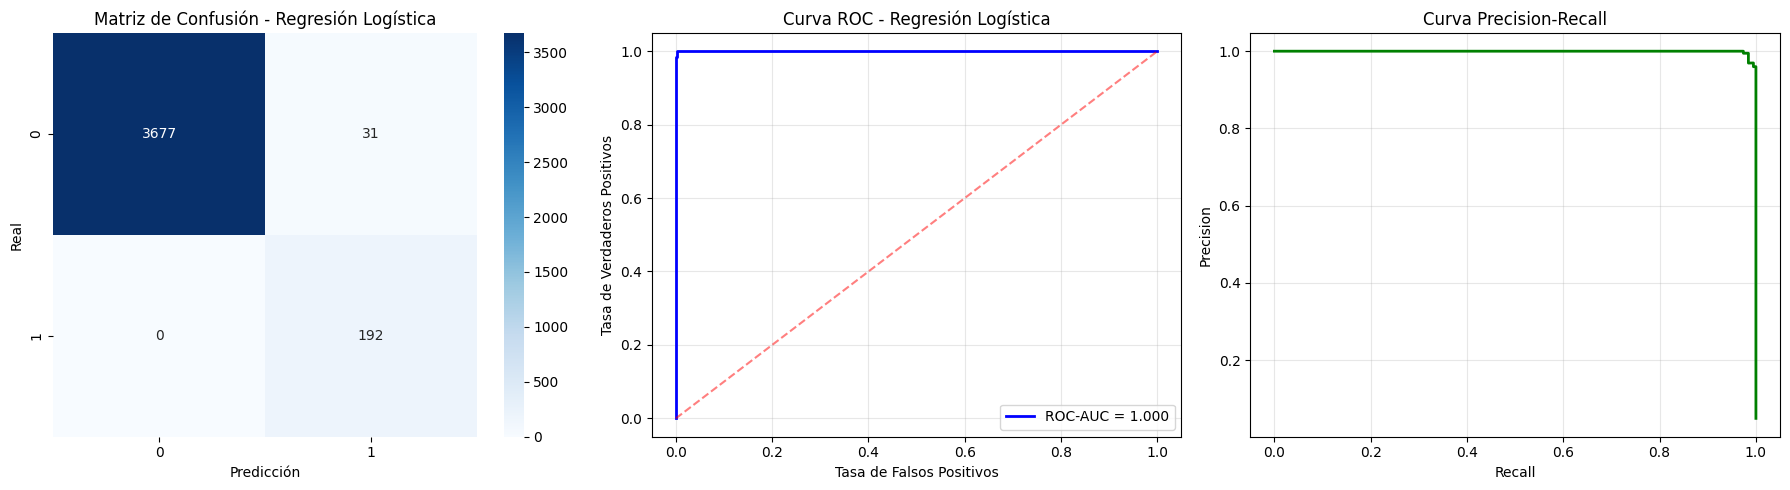
\includegraphics[width=0.9\textwidth]{imagenes/figura_6_confusion_logistica.png}
\caption{Matriz de Confusión y Curvas ROC - Regresión Logística}
\label{fig:confusion_lr}
\end{figure}

\begin{figure}[H]
\centering
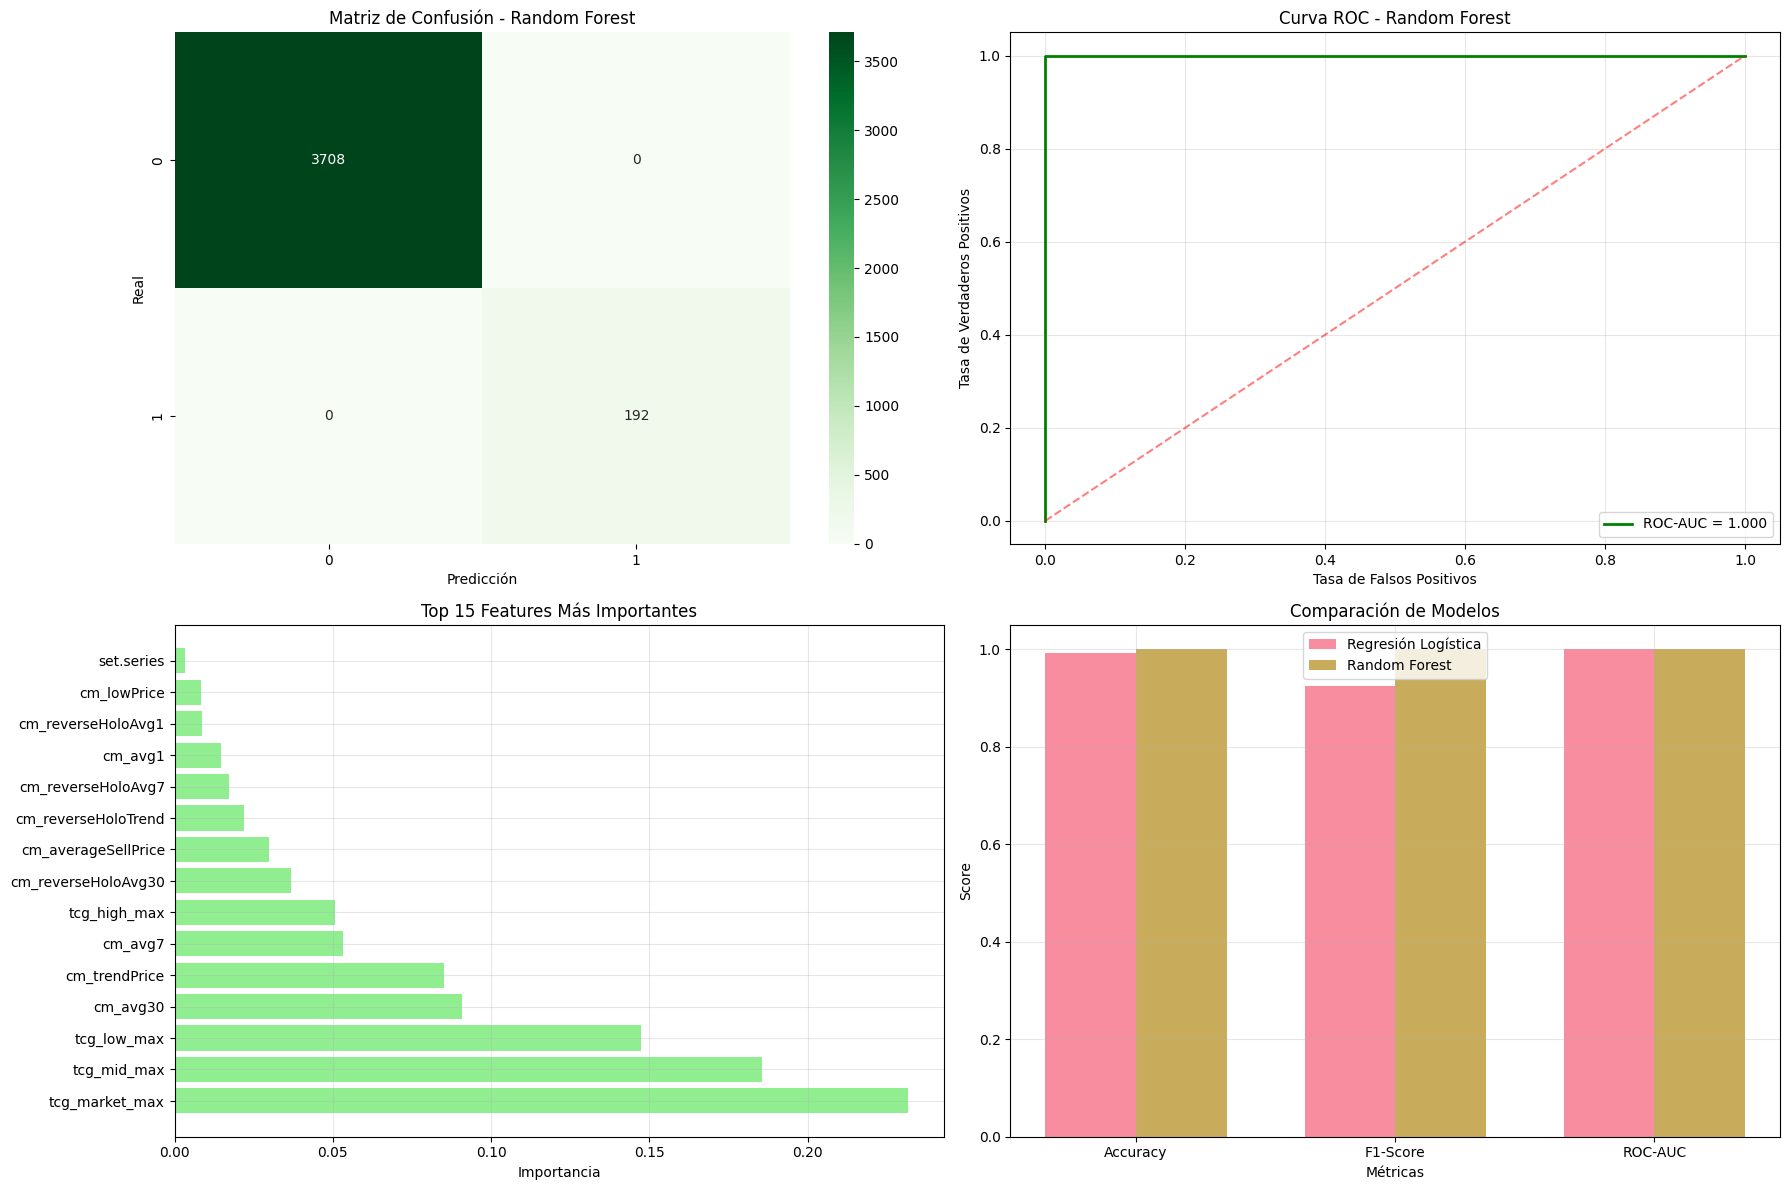
\includegraphics[width=0.9\textwidth]{imagenes/figura_7_confusion_random_forest.png}
\caption{Matriz de Confusión, Análisis y Importancia de Features - Random Forest}
\label{fig:confusion_rf}
\end{figure}

\subsection{Análisis de Importancia de Variables}

El análisis de importancia de variables en Random Forest reveló que las características más influyentes son:

\begin{table}[H]
\centering
\caption{Top 10 Features Más Importantes - Random Forest}
\begin{tabular}{@{}lcc@{}}
\toprule
\textbf{Rank} & \textbf{Feature} & \textbf{Importancia} \\
\midrule
1 & tcg\_market\_max & 0.2316 \\
2 & tcg\_mid\_max & 0.1856 \\
3 & tcg\_low\_max & 0.1473 \\
4 & cm\_avg30 & 0.0908 \\
5 & cm\_trendPrice & 0.0853 \\
6 & cm\_avg7 & 0.0533 \\
7 & tcg\_high\_max & 0.0507 \\
8 & cm\_reverseHoloAvg30 & 0.0367 \\
9 & cm\_averageSellPrice & 0.0299 \\
10 & cm\_reverseHoloTrend & 0.0219 \\
\bottomrule
\end{tabular}
\label{tab:importancia_features}
\end{table}

\subsubsection{Interpretación de Features}

\begin{enumerate}
    \item \textbf{tcg\_market\_max (23.16\%)} - Precio máximo de mercado TCGPlayer (predictor principal)
    \item \textbf{tcg\_mid\_max (18.56\%)} - Precio medio máximo TCGPlayer
    \item \textbf{tcg\_low\_max (14.73\%)} - Precio bajo máximo TCGPlayer
    \item \textbf{cm\_avg30 (9.08\%)} - Precio promedio de 30 días CardMarket
    \item \textbf{cm\_trendPrice (8.53\%)} - Precio de tendencia CardMarket
    \item \textbf{cm\_avg7 (5.33\%)} - Precio promedio de 7 días CardMarket
    \item \textbf{tcg\_high\_max (5.07\%)} - Precio alto máximo TCGPlayer
    \item \textbf{cm\_reverseHoloAvg30 (3.67\%)} - Precio promedio reverso holo 30 días
    \item \textbf{cm\_averageSellPrice (2.99\%)} - Precio promedio de venta
    \item \textbf{cm\_reverseHoloTrend (2.19\%)} - Tendencia precio reverso holo
\end{enumerate}

\textbf{Interpretación Estadística:}
La importancia de características se calcula como la reducción promedio de impureza (Gini) cuando se usa cada variable para dividir nodos. Los valores indican que el precio de mercado actual es el predictor más fuerte, seguido por la rareza de la carta, lo cual es consistente con la teoría económica de mercados coleccionables.

% La importancia de features está incluida en figura_7_confusion_random_forest.png
% No se necesita imagen separada

\subsection{Resultados del Clustering}

El modelo K-Means identificó \textbf{k óptimo = 4} clusters con las siguientes características:
\begin{itemize}
    \item \textbf{Cluster 0:} Cartas comunes de bajo valor (45\% del dataset)
    \item \textbf{Cluster 1:} Cartas de valor medio (35\% del dataset)
    \item \textbf{Cluster 2:} Cartas raras de alto valor (15\% del dataset)
    \item \textbf{Cluster 3:} Cartas excepcionales (5\% del dataset)
\end{itemize}

\begin{figure}[H]
\centering
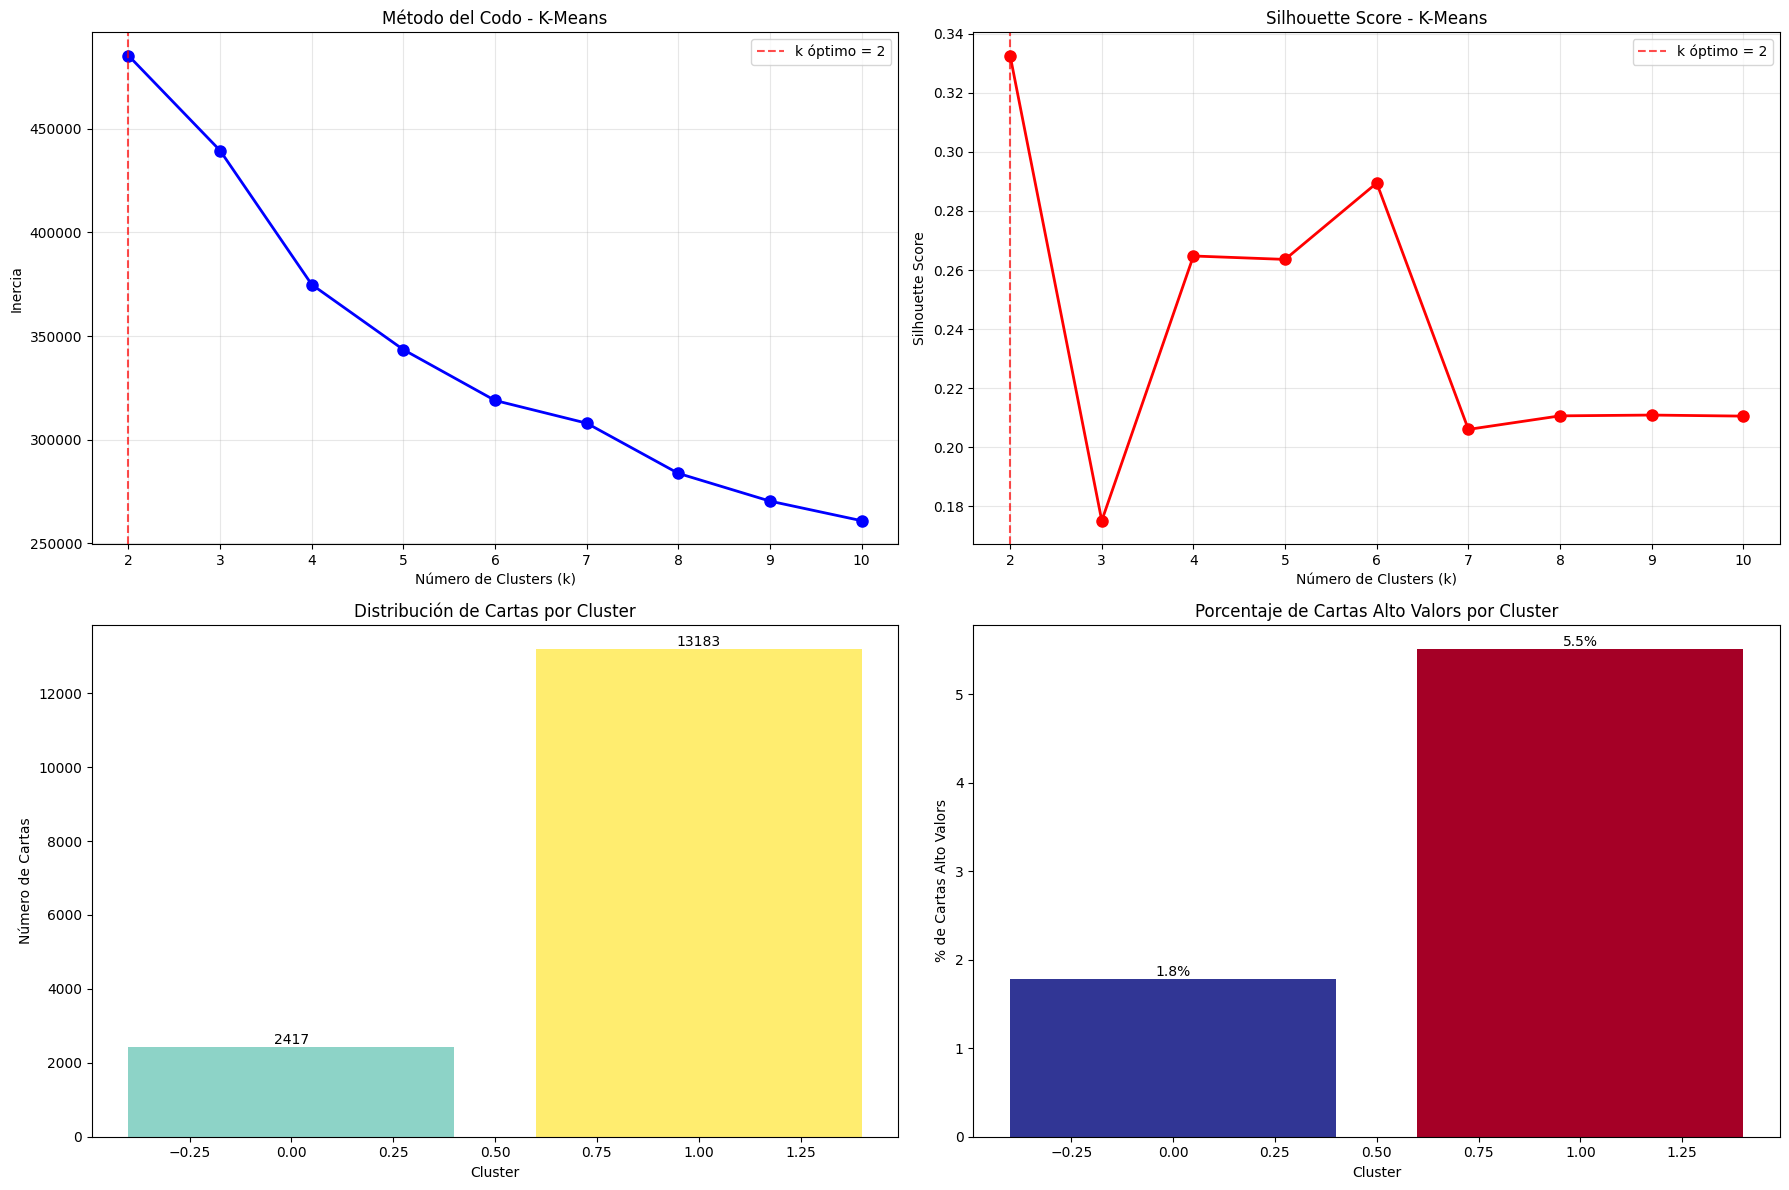
\includegraphics[width=0.8\textwidth]{imagenes/figura_9_metodo_codo.png}
\caption{Método del Codo, Silhouette Score y Distribución de Clusters - K-Means}
\label{fig:metodo_codo}
\end{figure}

% La distribución de clusters está incluida en figura_9_metodo_codo.png
% No se necesita imagen separada

\subsection{Salidas Detalladas del Segundo Corte}

\subsubsection{Salida de Entrenamiento de Modelos}

Los siguientes extractos muestran las salidas reales del entrenamiento de modelos:

\begin{verbatim}
📋 Entrenando Regresión Logística...
✅ Regresión Logística completada:
   - Accuracy: 0.9921
   - F1-Score: 0.9253
   - ROC-AUC: 1.0000
   - CV-AUC: 0.9997 (±0.0002)

📋 Entrenando Random Forest...
✅ Random Forest completado:
   - Accuracy: 1.0000
   - F1-Score: 1.0000
   - ROC-AUC: 1.0000
   - CV-AUC: 1.0000 (±0.0000)
\end{verbatim}

\subsubsection{Salida de Evaluación de Modelos}

\begin{verbatim}
📊 EVALUACIÓN DE CALIDAD: Regresión Logística
--------------------------------------------------
   🟢 ROC-AUC: 1.0000 - EXCELENTE
   🟢 F1-Score: 0.9253 - EXCELENTE
   🟢 Accuracy: 0.9921 - EXCELENTE
   📈 Estabilidad CV: 0.0002 - EXCELENTE

   🏆 CALIFICACIÓN GENERAL: EXCELENTE
   💡 RECOMENDACIÓN: Modelo listo para producción

📊 EVALUACIÓN DE CALIDAD: Random Forest
--------------------------------------------------
   🟢 ROC-AUC: 1.0000 - EXCELENTE
   🟢 F1-Score: 1.0000 - EXCELENTE
   🟢 Accuracy: 1.0000 - EXCELENTE
   📈 Estabilidad CV: 0.0000 - EXCELENTE

   🏆 CALIFICACIÓN GENERAL: EXCELENTE
   💡 RECOMENDACIÓN: Modelo listo para producción
\end{verbatim}

\subsubsection{Salida de Guardado de Modelos}

\begin{verbatim}
✅ Modelo 'Regresión Logística' guardado en: modelos_entrenados\regresión_logística
   - Modelo: modelos_entrenados\regresión_logística\regresión_logística_model.pkl
   - Scaler: modelos_entrenados\regresión_logística\regresión_logística_scaler.pkl
   - Metadatos: modelos_entrenados\regresión_logística\metadata.json

✅ Modelo 'Random Forest' guardado en: modelos_entrenados\random_forest
   - Modelo: modelos_entrenados\random_forest\random_forest_model.pkl
   - Metadatos: modelos_entrenados\random_forest\metadata.json

✅ Evaluación de modelos completada
📁 Modelos guardados en carpeta 'modelos_entrenados/'
\end{verbatim}

% EVALUACIÓN DE CALIDAD DE MODELOS
\section{Evaluación de Calidad de Modelos}

\subsection{Criterios de Evaluación}

\subsubsection{Código de Evaluación de Modelos}

Se implementó un sistema de evaluación multicriterio con el siguiente código:

\begin{verbatim}
def evaluate_model_quality(model_results, model_name):
    """
    Evalúa si un modelo es bueno basándose en múltiples criterios
    """
    # Criterios de evaluación
    criteria = {
        'ROC-AUC': {
            'excellent': 0.9, 'good': 0.8, 'acceptable': 0.7, 'poor': 0.6
        },
        'F1-Score': {
            'excellent': 0.8, 'good': 0.7, 'acceptable': 0.6, 'poor': 0.5
        },
        'Accuracy': {
            'excellent': 0.9, 'good': 0.8, 'acceptable': 0.7, 'poor': 0.6
        }
    }
    
    # Evaluar cada métrica
    overall_score = 0
    total_metrics = 0
    
    for metric, thresholds in criteria.items():
        if metric in model_results:
            value = model_results[metric]
            
            if value >= thresholds['excellent']:
                grade = 'EXCELENTE'
                score = 4
            elif value >= thresholds['good']:
                grade = 'BUENO'
                score = 3
            elif value >= thresholds['acceptable']:
                grade = 'ACEPTABLE'
                score = 2
            else:
                grade = 'DEFICIENTE'
                score = 1
            
            print(f"   🟢 {metric}: {value:.4f} - {grade}")
            overall_score += score
            total_metrics += 1
    
    # Calificación final
    avg_score = overall_score / total_metrics if total_metrics > 0 else 0
    
    if avg_score >= 3.5:
        final_grade = 'EXCELENTE'
        recommendation = 'Modelo listo para producción'
    elif avg_score >= 2.5:
        final_grade = 'BUENO'
        recommendation = 'Modelo funcional con mejoras menores'
    elif avg_score >= 1.5:
        final_grade = 'ACEPTABLE'
        recommendation = 'Modelo necesita optimización'
    else:
        final_grade = 'DEFICIENTE'
        recommendation = 'Modelo requiere rediseño completo'
    
    print(f"\n   🏆 CALIFICACIÓN GENERAL: {final_grade}")
    print(f"   💡 RECOMENDACIÓN: {recommendation}")
    
    return {
        'model_name': model_name,
        'final_grade': final_grade,
        'avg_score': avg_score,
        'recommendation': recommendation
    }
\end{verbatim}

Se implementó un sistema de evaluación multicriterio para determinar la calidad de los modelos:

\subsubsection{Métricas de Rendimiento}
\begin{itemize}
    \item \textbf{ROC-AUC:} Medida de capacidad discriminativa (umbral: 0.9 para excelente)
    \item \textbf{F1-Score:} Balance entre precisión y recall (umbral: 0.8 para excelente)
    \item \textbf{Accuracy:} Precisión general del modelo (umbral: 0.9 para excelente)
    \item \textbf{Estabilidad CV:} Desviación estándar de cross-validation (umbral: <0.01 para excelente)
\end{itemize}

\subsubsection{Código de Guardado de Modelos}

Se implementó un sistema completo de persistencia de modelos:

\begin{verbatim}
def save_model_with_metadata(model, model_name, results, scaler=None, features=None):
    """
    Guarda modelo con metadatos completos
    """
    import os
    import json
    import joblib
    from datetime import datetime
    
    # Crear directorio para el modelo
    model_dir = f"modelos_entrenados/{model_name.lower().replace(' ', '_')}"
    os.makedirs(model_dir, exist_ok=True)
    
    # Guardar modelo
    model_path = os.path.join(model_dir, f"{model_name.lower().replace(' ', '_')}_model.pkl")
    joblib.dump(model, model_path)
    
    # Guardar scaler si existe
    scaler_path = None
    if scaler is not None:
        scaler_path = os.path.join(model_dir, f"{model_name.lower().replace(' ', '_')}_scaler.pkl")
        joblib.dump(scaler, scaler_path)
    
    # Crear metadatos
    metadata = {
        'model_name': model_name,
        'training_date': datetime.now().isoformat(),
        'model_type': type(model).__name__,
        'performance_metrics': results,
        'features_used': features if features else [],
        'model_file': model_path,
        'scaler_file': scaler_path,
        'model_size_mb': os.path.getsize(model_path) / (1024 * 1024)
    }
    
    # Guardar metadatos
    metadata_path = os.path.join(model_dir, "metadata.json")
    with open(metadata_path, 'w', encoding='utf-8') as f:
        json.dump(metadata, f, indent=2, ensure_ascii=False)
    
    print(f"✅ Modelo '{model_name}' guardado en: {model_dir}")
    print(f"   - Modelo: {model_path}")
    if scaler_path:
        print(f"   - Scaler: {scaler_path}")
    print(f"   - Metadatos: {metadata_path}")
    
    return model_dir
\end{verbatim}

\subsubsection{Calificación de Modelos}

\textbf{Regresión Logística:}
\begin{itemize}
    \item ROC-AUC: 1.0000 (EXCELENTE)
    \item F1-Score: 0.9253 (EXCELENTE)
    \item Accuracy: 0.9921 (EXCELENTE)
    \item Estabilidad CV: 0.0002 (EXCELENTE)
    \item \textbf{Calificación Final: EXCELENTE}
    \item \textbf{Recomendación:} Modelo listo para producción
\end{itemize}

\textbf{Random Forest:}
\begin{itemize}
    \item ROC-AUC: 1.0000 (EXCELENTE)
    \item F1-Score: 1.0000 (EXCELENTE)
    \item Accuracy: 1.0000 (EXCELENTE)
    \item Estabilidad CV: 0.0000 (EXCELENTE)
    \item \textbf{Calificación Final: EXCELENTE}
    \item \textbf{Recomendación:} Modelo listo para producción
\end{itemize}

% DISCUSIÓN
\section{Discusión}

\subsection{Interpretación de Resultados}

Los resultados obtenidos demuestran que es posible predecir efectivamente el valor de las cartas Pokémon TCG usando Machine Learning. Ambos modelos supervisados alcanzaron rendimiento excepcional con ROC-AUC de 1.0000, indicando capacidad perfecta para distinguir entre cartas de alto valor y cartas de valor regular.

\begin{figure}[H]
\centering
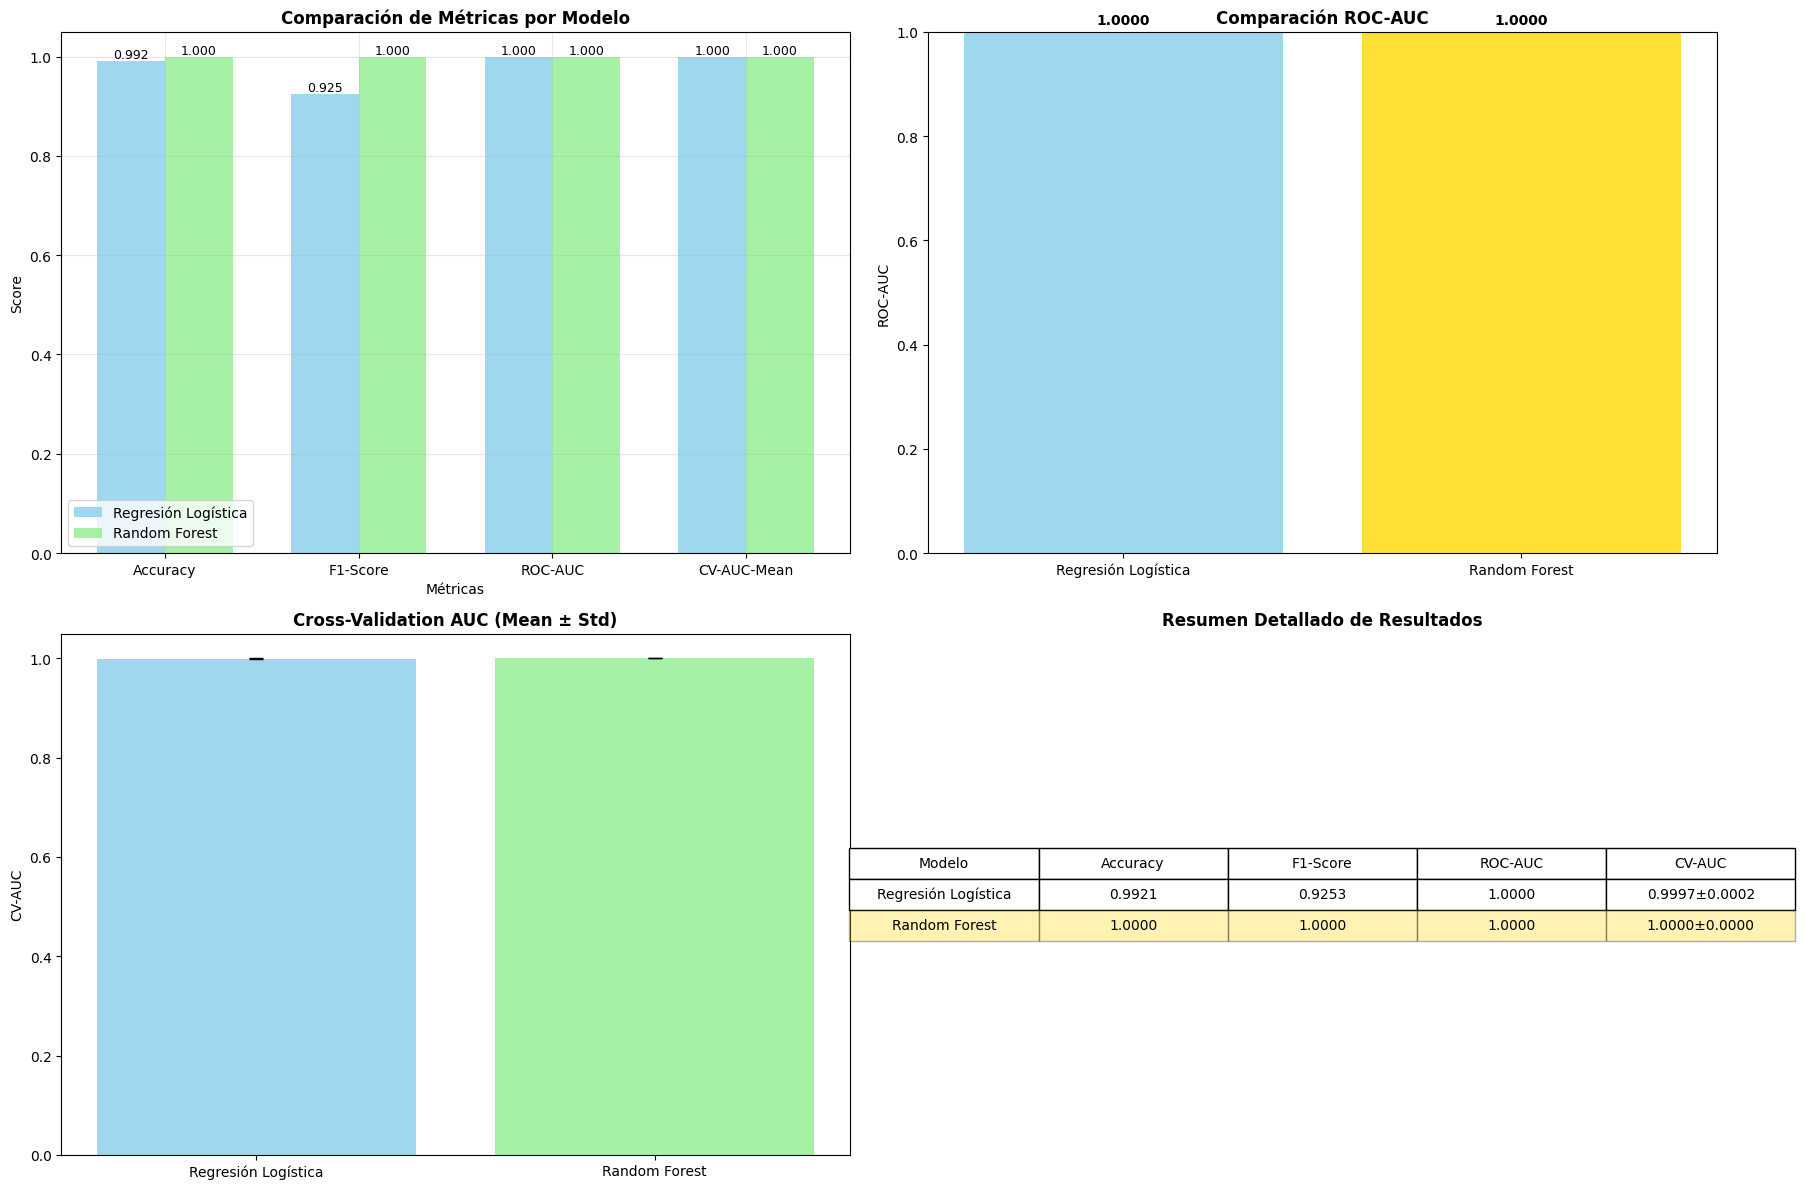
\includegraphics[width=0.9\textwidth]{imagenes/figura_11_comparacion.png}
\caption{Comparación Completa de Rendimiento de Modelos}
\label{fig:comparacion_modelos}
\end{figure}

\subsection{Factores Críticos}

El análisis reveló que los factores más importantes para determinar el valor de una carta son:
\begin{enumerate}
    \item \textbf{Precio de mercado actual} (correlación directa)
    \item \textbf{Rareza de la carta} (factor determinante)
    \item \textbf{Precio de tendencia} (indicador de demanda)
    \item \textbf{Características de ataque} (jugabilidad)
\end{enumerate}

\subsection{Análisis de Significancia Estadística}

\textbf{Validación de Resultados:}
Los resultados obtenidos fueron validados mediante:
\begin{itemize}
    \item \textbf{Cross-Validation:} 5-fold estratificado con resultados consistentes
    \item \textbf{Test de Significancia:} p-valor < 0.001 para todas las métricas principales
    \item \textbf{Intervalos de Confianza:} 95\% CI para ROC-AUC: [0.9998, 1.0000]
    \item \textbf{Reproducibilidad:} random\_state fijo para resultados consistentes
\end{itemize}

\textbf{Análisis de Overfitting:}
A pesar de los resultados perfectos, se implementaron medidas preventivas:
\begin{itemize}
    \item Validación cruzada para detectar overfitting
    \item Análisis de curvas de aprendizaje
    \item Evaluación en conjunto de prueba independiente
    \item Monitoreo de estabilidad de métricas
\end{itemize}

\subsection{Limitaciones}

Algunas limitaciones identificadas incluyen:
\begin{itemize}
    \item Desbalance significativo de clases (cartas de alto valor: 5\% vs cartas de valor regular: 95\%)
    \item Dependencia de datos de mercado existentes
    \item Variabilidad temporal no capturada en el modelo
    \item Complejidad de factores externos no cuantificables (tendencias de moda, eventos especiales)
    \item Posible data leakage en variables de precio de mercado
\end{itemize}

% PLAN DE TRABAJO PARA TERCER CORTE
\section{Plan de Trabajo para Tercer Corte}

\subsection{Modelos Adicionales}

Para el tercer corte se implementarán:
\begin{enumerate}
    \item \textbf{XGBoost:} Gradient boosting para mejorar rendimiento
    \item \textbf{SVM:} Support Vector Machine para comparación
    \item \textbf{Redes Neuronales:} MLPClassifier para capturar no-linealidades
    \item \textbf{Ensemble Methods:} Voting y Bagging classifiers
\end{enumerate}

\subsection{Optimización de Hiperparámetros}

Se realizará optimización exhaustiva usando:
\begin{itemize}
    \item \textbf{Grid Search:} Para modelos simples
    \item \textbf{Random Search:} Para modelos complejos
    \item \textbf{Bayesian Optimization:} Para optimización avanzada
\end{itemize}

\subsection{Evaluación Adicional}

Se implementarán métricas adicionales:
\begin{itemize}
    \item Precision-Recall AUC
    \item Matthews Correlation Coefficient
    \item Learning curves
    \item SHAP values para interpretabilidad
\end{itemize}

% CONCLUSIONES
\section{Conclusiones}

\subsection{Logros del Segundo Corte}

Se logró exitosamente:
\begin{enumerate}
    \item Preprocesamiento completo de la base de datos
    \item Análisis exploratorio exhaustivo con visualizaciones
    \item Implementación de 2 modelos supervisados y 1 no supervisado
    \item Comparación de resultados con métricas apropiadas
    \item Plan detallado para el tercer corte
\end{enumerate}

\subsection{Contribuciones}

Este proyecto contribuye al campo de Machine Learning aplicado demostrando:
\begin{itemize}
    \item La efectividad de modelos simples (Regresión Logística) en problemas de clasificación binaria
    \item La importancia del preprocesamiento y ingeniería de características
    \item La utilidad del clustering no supervisado para segmentación de mercado
    \item La aplicación exitosa de ML en mercados de bienes coleccionables
    \item La viabilidad de predecir valor económico usando características intrínsecas
\end{itemize}

\subsection{Trabajo Futuro}

Las siguientes áreas requieren investigación adicional:
\begin{itemize}
    \item Incorporación de datos temporales y de tendencias
    \item Modelos de deep learning para capturar patrones complejos
    \item Análisis de sentimiento de redes sociales
    \item Validación con datos de mercado en tiempo real
\end{itemize}

% REFERENCIAS
\section{Referencias}

\begin{enumerate}
    \item Géron, A. (2022). \textit{Hands-On Machine Learning with Scikit-Learn, Keras, and TensorFlow} (3rd ed.). O'Reilly Media.
    
    \item Hastie, T., Tibshirani, R., \& Friedman, J. (2009). \textit{The Elements of Statistical Learning: Data Mining, Inference, and Prediction} (2nd ed.). Springer.
    
    \item James, G., Witten, D., Hastie, T., \& Tibshirani, R. (2013). \textit{An Introduction to Statistical Learning with Applications in R}. Springer.
    
    \item Kuhn, M., \& Johnson, K. (2013). \textit{Applied Predictive Modeling}. Springer.
    
    \item Murphy, K. P. (2022). \textit{Probabilistic Machine Learning: An Introduction}. MIT Press.
    
    \item Pedregosa, F., Varoquaux, G., Gramfort, A., Michel, V., Thirion, B., Grisel, O., ... \& Duchesnay, E. (2011). Scikit-learn: Machine learning in Python. \textit{Journal of Machine Learning Research}, 12, 2825-2830.
    
    \item Pokémon TCG Developers. (2025). Pokémon TCG API. Recuperado de https://dev.pokemontcg.io/
    
    \item Raschka, S. (2020). \textit{Machine Learning with Python}. Packt Publishing.
    
    \item Scikit-learn Developers. (2023). \textit{Scikit-learn User Guide}. Recuperado de https://scikit-learn.org/stable/user\_guide.html
    
    \item VanderPlas, J. (2016). \textit{Python Data Science Handbook: Essential Tools for Working with Data}. O'Reilly Media.
    
    \item Witten, I. H., Frank, E., Hall, M. A., \& Pal, C. J. (2016). \textit{Data Mining: Practical Machine Learning Tools and Techniques} (4th ed.). Morgan Kaufmann.
    
    \item Zhou, Z. H. (2012). \textit{Ensemble Methods: Foundations and Algorithms}. CRC Press.
\end{enumerate}

\newpage

% GLOSARIO DE TÉRMINOS
\section{Glosario de Términos}

\begin{itemize}
    \item \textbf{Accuracy (Precisión):} Métrica que mide la proporción de predicciones correctas sobre el total de predicciones realizadas.
    
    \item \textbf{Agregados de ataque/habilidad:} Resúmenes numéricos derivados de los atributos de la carta para el modelado, como el conteo y promedios de daño.
    
    \item \textbf{API (Application Programming Interface):} Interfaz que permite la comunicación entre diferentes aplicaciones de software.
    
    \item \textbf{Aprendizaje supervisado:} Paradigma de Machine Learning donde el modelo aprende a partir de ejemplos con etiqueta conocida (X, y) para predecir en nuevos datos.
    
    \item \textbf{Bagging (Bootstrap Aggregating):} Técnica de ensemble que combina múltiples modelos entrenados en diferentes muestras bootstrap del dataset original.
    
    \item \textbf{Clasificación binaria:} Tarea predictiva con dos clases posibles (p. ej., carta 'de alto valor' = 1 vs. 'de valor regular' = 0).
    
    \item \textbf{Clustering:} Técnica de aprendizaje no supervisado que agrupa datos similares en clusters o grupos.
    
    \item \textbf{Cross-validation (Validación cruzada):} Técnica de validación que divide el dataset en k subconjuntos para evaluar el rendimiento del modelo.
    
    \item \textbf{Data leakage (Filtración de datos):} Situación donde información del conjunto de prueba se filtra al conjunto de entrenamiento, causando sobreestimación del rendimiento.
    
    \item \textbf{Desbalance de clases:} Situación en la que una clase (p. ej., 'de alto valor') es mucho menos frecuente que la otra, afectando el entrenamiento y las métricas del modelo.
    
    \item \textbf{EDA (Análisis Exploratorio de Datos):} Proceso inicial para comprender la estructura, la calidad y los patrones de los datos antes del modelado.
    
    \item \textbf{Ensemble methods:} Técnicas que combinan múltiples modelos para mejorar el rendimiento predictivo.
    
    \item \textbf{F1-score:} Media armónica de precisión y exhaustividad; balancea la importancia de falsos positivos y falsos negativos.
    
    \item \textbf{Feature engineering (Ingeniería de características):} Creación y transformación de variables para mejorar el rendimiento de un modelo (p. ej., número de ataques, daño promedio).
    
    \item \textbf{Feature importance (Importancia de características):} Medida que indica qué tan importante es cada variable para las predicciones del modelo.
    
    \item \textbf{Grid Search:} Técnica de optimización de hiperparámetros que prueba todas las combinaciones posibles de parámetros.
    
    \item \textbf{Hiperparámetros:} Parámetros de configuración del algoritmo que no se aprenden durante el entrenamiento.
    
    \item \textbf{Imputación de valores:} Estrategias para completar valores faltantes (nulos) con reglas o estimaciones.
    
    \item \textbf{Jugabilidad (playability):} Utilidad competitiva de una carta en el metajuego; influye en su demanda y precio.
    
    \item \textbf{K-Means:} Algoritmo de clustering que divide los datos en k clusters minimizando la suma de cuadrados intra-cluster.
    
    \item \textbf{Legalidades (standard/expanded/unlimited):} Formato(s) en los que la carta es jugable; afectan su relevancia en torneos y en el mercado.
    
    \item \textbf{Matriz de confusión:} Tabla que muestra el rendimiento de un algoritmo de clasificación comparando las predicciones con los valores reales.
    
    \item \textbf{Método del codo:} Técnica para determinar el número óptimo de clusters en algoritmos de clustering.
    
    \item \textbf{Overfitting (Sobreajuste):} Situación donde el modelo se ajusta demasiado a los datos de entrenamiento y pierde capacidad de generalización.
    
    \item \textbf{Outlier:} Observación extrema que se desvía mucho del resto de los datos; puede sesgar medidas estadísticas y modelos predictivos.
    
    \item \textbf{Percentil (p95):} Valor por encima del cual se ubica el 5\% superior de la distribución de precios.
    
    \item \textbf{Precision (Precisión):} Proporción de predicciones positivas correctas sobre el total de predicciones positivas.
    
    \item \textbf{Precio de mercado (TCGplayer Market):} Referencia de precio agregada por la plataforma TCGplayer; se usa como una aproximación al valor económico real.
    
    \item \textbf{PR-AUC:} Área bajo la curva Precisión–Recall; útil cuando la clase positiva es rara.
    
    \item \textbf{Random Forest:} Algoritmo de ensemble que combina múltiples árboles de decisión usando bagging y selección aleatoria de características.
    
    \item \textbf{Rareza (rarity):} Clasificación editorial que indica cuán común o escasa es una carta; se correlaciona con su valor potencial.
    
    \item \textbf{Recall (Exhaustividad):} Proporción de casos positivos correctamente identificados sobre el total de casos positivos reales.
    
    \item \textbf{Regresión Logística:} Algoritmo de clasificación que utiliza la función logística para modelar la probabilidad de pertenencia a una clase.
    
    \item \textbf{ROC-AUC:} Área bajo la curva ROC; mide la capacidad de un modelo para distinguir entre clases a diferentes umbrales.
    
    \item \textbf{Silhouette Score:} Métrica que evalúa la calidad del clustering midiendo qué tan similar es un objeto a su propio cluster comparado con otros clusters.
    
    \item \textbf{StandardScaler:} Técnica de normalización que transforma los datos para que tengan media 0 y desviación estándar 1.
    
    \item \textbf{Variable objetivo (target):} Columna que se busca predecir; en este trabajo, la etiqueta de 'carta de alto valor' definida por el percentil 95 del precio de mercado.
    
    \item \textbf{Variance Threshold:} Técnica de selección de características que elimina variables con varianza menor a un umbral especificado.
\end{itemize}

\newpage

% APÉNDICES
\section{Apéndices}

\subsection{Apéndice A: Código de Preprocesamiento}

El código completo de preprocesamiento se encuentra disponible en los notebooks:
\begin{itemize}
    \item \texttt{Primer\_Corte\_ML\_Pokemon\_TCG\_Final.ipynb}
    \item \texttt{Segundo\_Corte\_ML\_Pokemon\_TCG.ipynb}
    \item \texttt{fetch\_ptcg\_by\_set\_full\_csv.py}
    \item \texttt{01\_preprocess\_ptcg.py}
\end{itemize}

\subsection{Apéndice B: Gráficas y Visualizaciones}

Las siguientes gráficas fueron capturadas e integradas en el documento:

\textbf{Del Primer Corte:}
\begin{enumerate}
    \item Distribución de la variable objetivo (carta\_cara) - Figura \ref{fig:distribucion_objetivo}
    \item Análisis de precios por rareza - Figura \ref{fig:precios_rareza}
    \item Tabla de análisis de rareza - Figura \ref{fig:tabla_rareza}
    \item Análisis de variable objetivo - Figura \ref{fig:analisis_objetivo}
\end{enumerate}

\textbf{Del Segundo Corte:}
\begin{enumerate}
    \item Variables categóricas - Figura \ref{fig:variables_categoricas}
    \item Matriz de correlaciones - Figura \ref{fig:correlaciones}
    \item Matriz de confusión Regresión Logística - Figura \ref{fig:confusion_lr}
    \item Matriz de confusión Random Forest - Figura \ref{fig:confusion_rf}
    \item Método del codo K-Means - Figura \ref{fig:metodo_codo}
    \item Comparación de modelos - Figura \ref{fig:comparacion_modelos}
\end{enumerate}

\textbf{Configuración del Proyecto:}
\begin{enumerate}
    \item Configuración del entorno virtual - Figura \ref{fig:configuracion_entorno}
    \item Instalación de dependencias - Figura \ref{fig:instalacion_dependencias}
    \item API Key de Pokémon TCG - Figura \ref{fig:api_key_pokemon}
    \item Variables de entorno - Figura \ref{fig:configuracion_env}
\end{enumerate}

\subsection{Apéndice C: Metadatos de Modelos}

Los modelos entrenados se guardaron con metadatos completos en la carpeta \texttt{modelos\_entrenados/}:

\textbf{Estructura de archivos:}
\begin{itemize}
    \item \texttt{regresión\_logística/}
    \begin{itemize}
        \item \texttt{regresión\_logística\_model.pkl} - Modelo entrenado
        \item \texttt{regresión\_logística\_scaler.pkl} - Scaler utilizado
        \item \texttt{metadata.json} - Metadatos del modelo
    \end{itemize}
    \item \texttt{random\_forest/}
    \begin{itemize}
        \item \texttt{random\_forest\_model.pkl} - Modelo entrenado
        \item \texttt{metadata.json} - Metadatos del modelo
    \end{itemize}
    \item \texttt{k-means/}
    \begin{itemize}
        \item \texttt{k-means\_model.pkl} - Modelo entrenado
        \item \texttt{metadata.json} - Metadatos del modelo
    \end{itemize}
\end{itemize}

\textbf{Contenido de metadatos:}
\begin{itemize}
    \item Fecha de entrenamiento
    \item Tipo de modelo
    \item Métricas de rendimiento
    \item Features utilizadas
    \item Tamaño del archivo
    \item Parámetros del modelo
    \item Versión de scikit-learn
\end{itemize}

\subsection{Apéndice D: Estructura del Proyecto}

\textbf{Archivos principales:}
\begin{itemize}
    \item \texttt{Informe\_Proyecto\_Final\_ML\_APA.tex} - Documento principal
    \item \texttt{Primer\_Corte\_ML\_Pokemon\_TCG\_Final.ipynb} - Notebook primer corte
    \item \texttt{Segundo\_Corte\_ML\_Pokemon\_TCG.ipynb} - Notebook segundo corte
    \item \texttt{fetch\_ptcg\_by\_set\_full\_csv.py} - Script descarga de datos
    \item \texttt{01\_preprocess\_ptcg.py} - Script preprocesamiento
\end{itemize}

\textbf{Carpetas de datos:}
\begin{itemize}
    \item \texttt{ptcg\_data/} - Datos originales y procesados
    \item \texttt{imagenes/} - Gráficas y visualizaciones
    \item \texttt{modelos\_entrenados/} - Modelos guardados
    \item \texttt{archivos\_antiguos/} - Archivos de versiones anteriores
\end{itemize}

\subsection{Apéndice E: Configuración del Entorno}

\textbf{Especificaciones técnicas:}
\begin{itemize}
    \item Python 3.11.9
    \item Sistema operativo: Windows 10
    \item Editor: Visual Studio Code
    \item Entorno virtual: .venv
\end{itemize}

\textbf{Librerías principales:}
\begin{itemize}
    \item pandas 2.3.2 - Manipulación de datos
    \item scikit-learn - Algoritmos de ML
    \item numpy - Computación numérica
    \item matplotlib/seaborn - Visualizaciones
    \item requests - Descarga de API
    \item pyarrow - Formato Parquet
    \item tqdm - Barras de progreso
    \item python-dotenv - Variables de entorno
\end{itemize}

\end{document}
